\documentclass[8pt, compress]{beamer}
\usepackage[utf8]{inputenc}
\usepackage{graphicx}
\usepackage{amsmath}
\usepackage{mathtools}
\usepackage{amssymb}
\usepackage{bbm}
\usepackage{tikz}
\usetikzlibrary{positioning}


\usetheme{CambridgeUS}
\usecolortheme{beaver}

\setbeamertemplate{footline}
{
  \hbox{\begin{beamercolorbox}[wd=1\paperwidth,ht=2.25ex,dp=1ex,right]{framenumber}%
      \usebeamerfont{framenumber}\insertframenumber{} / \inserttotalframenumber\hspace*{2ex}
    \end{beamercolorbox}}%
  \vskip0pt%
}

\setbeamercolor{block title}{use=structure,fg=white,bg=red!75!black}
\setbeamercolor{block body}{use=structure,fg=black,bg=gray!10}

\useoutertheme{miniframes}

%%% For XOR Symbol
\tikzset{XOR/.style={draw,circle,append after command={
        [shorten >=\pgflinewidth, shorten <=\pgflinewidth,]
        (\tikzlastnode.north) edge (\tikzlastnode.south)
        (\tikzlastnode.east) edge (\tikzlastnode.west)
        }
    }
}
%%% For changing color
\usetikzlibrary{overlay-beamer-styles}

\definecolor{mycolor}{rgb}{231,231,233}

\title{\Large Polar Codes}
\author{\large Aayush Rajesh, Ronil Mandavia}
\institute{\large Department of Electrical Engineering \\ \large IIT Bombay}
\date{}

\begin{document}

\frame{\titlepage}

\begin{frame}{Outline}
    \tableofcontents
\end{frame}

\section{Introduction}

\begin{frame}{Overview}
\begin{itemize}
    \item<1-> Polar Codes were introduced by Erdal Arıkan in \cite{5075875}, and are constructed by exploiting a phenomenon known as \textbf{channel polarization}.
    \item<2-> It can be shown that these codes achieve Shannon's Capacity.
    \item<3-> We shall look to motivate the polarization phenomenon to understand how these codes achieve capacity. Efficient encoding and decoding procedures shall also be covered.
\end{itemize}
\end{frame}

\begin{frame}
\frametitle{Information Theoretic Measures}
\begin{itemize}
    
\item<1-> \textbf{Entropy:} Entropy measures the average uncertainty in a random variable.

$$
H(X) = - \sum_{x \in \mathcal{X}} p(x) \log p(x)
$$ 

\onslide<2->{
$$
H(Y|X) = - \sum_{x \in \mathcal{X}} \sum_{y \in \mathcal{Y}} p(x, y) \log p(y|x)
$$
}

\item<3-> \textbf{Mutual Information:} The reduction in uncertainty in one random variable due to knowledge of another.

$$
I(X; Y) = H(X) - H(X|Y) \onslide<4->{ = H(Y) - H(Y|X)}
$$

\item<5-> \textbf{Chain Rule:} $$I(X, Y; Z) = I(X; Z) + I(Y; Z|X)$$

\end{itemize}

\end{frame}

\begin{frame}{The Channel}
\onslide<1->{
\begin{center}
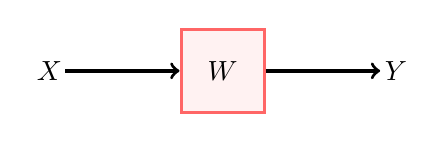
\begin{tikzpicture}[channel/.style={rectangle, draw=red!60, fill=red!5, very thick, minimum size=30}]
    \node[channel](channel){$W$};
    \node[] at (-2.2,0) {$X$};
    \node[] at (2.2,0) {$Y$};
    \draw[->, very thick] (-2,0) to (channel.west); 
    \draw[->, very thick] (channel.east) to (2, 0);
\end{tikzpicture}
\end{center}
}

\begin{itemize}
    \item<1-> Channel $W : \mathcal{X} \to \mathcal{Y}$, characterized by \textbf{transition probabilities} $W(y|x)$.
    \item<2-> The maximum rate of reliable communication over this B-DMC\footnote<2->{Binary-Discrete Memoryless Channel} is the \textbf{capacity} and is given by
    $$
    C = \max_{p(x)} I(X; Y)
    $$
    \item<3-> There are two classes for which analysis of communication is trivial
    \begin{itemize}
        \item<3-> Perfect Channels: $C = 1$
        \item<3-> Useless Channels: $C = 0$
    \end{itemize}
\end{itemize}

\end{frame}

\begin{frame}{Channel Capacity}
\onslide<1->{A simple analysis of channel capacity can be undertaken for the BEC(p) channel. We have $W(0|0) = W(1|1) = 1-p$ and $W(\textcolor{red}{?}|0) =W(\textcolor{red}{?}|1) = p$. The mutual information of the channel can be evaluated as}

\begin{equation*}
\begin{split}
\onslide<2->{I(X;Y) &= H(X) - H(X|Y)\\}
\onslide<3->{ &= H(X) - p_Y(\textcolor{red}{?})H(X|\textcolor{red}{?}) - p_Y(0)H(X|0) - p_Y(1)H(X|1)\\}
\uncover<4->{ \alt<5->{&= (1-p)H(X)}{&= H(X) - pH(X) - 0 - 0}}
\end{split}
\end{equation*}

\onslide<6->{This quantity is maximized when $X \sim \text{Ber}\left(\frac{1}{2}\right)$, giving us $C = 1 - p$ for a BEC(p) channel. Through a similar analysis, we can obtain that $C = 1 - H(p)$ for a BSC(p) channel.}
\end{frame}

\section{Polarization}

\begin{frame}{Combining Channels}

\begin{columns}
    \begin{column}{0.6\linewidth}
        \begin{itemize}
            \item<1-> We can denote $X_1 = U_1 \oplus U_2$ and $X_2 = U_2$. There is an invertible transformation between $(U_1, U_2)$ and ($X_1, X_2)$.
            \item<2-> The capacity of this joint ensemble is
            \begin{equation*}
            \begin{split}
            2C(W) &= I(X_1 X_2; Y_1 Y_2) = I(U_1 U_2; Y_1 Y_2)\\
            \onslide<3->{ &= I(U_1; Y_1 Y_2) + I(U_2; Y_1 Y_2 | U_1)\\}
            \onslide<4->{ &= I(U_1; Y_1 Y_2) + I(U_2; Y_1 Y_2 U_1)\\}
            \only<5>{ &= C(W^-) + C(W^+)\\}
            \only<6>{ &= C(\textcolor{red}{W^-}) + C(W^+)\\}
            \only<7>{ &= C(W^-) + C(\textcolor{green}{W^+})\\}
            \onslide<8->{ &= C(W^-) + C(W^+)\\}
            \end{split}
            \end{equation*}
        \end{itemize}
    \end{column}
    \begin{column}{0.37\linewidth}
        \begin{tikzpicture}[channel/.style={rectangle, draw=black!80, fill=white!5, very thick, minimum size=30}, scale=0.8, every node/.style={scale=0.8}]
            \node[channel](channel1){$W$};
            \node[channel](channel2) at (0, -1.5) {$W$};
            \alt<7>{\node[] at (-2.5,0) {\textcolor{green}{$U_1$}}}{\node[] at (-2.5,0) {$U_1$}};
            %\alt<7>{\node[] at (-2.5,0) {\textcolor{green}{$U_1$}}}{\node[] at (-2.5,0) {$U_1$}};
            \alt<6>{\node[] at (2,0) {\textcolor{red}{$Y_1$}}}{\alt<7>{\node[] at (2,0) {\textcolor{green}{$Y_1$}}}{\node[] at (2,0) {$Y_1$}}};
            \alt<6>{\node[] at (-2.5,-1.5) {\textcolor{black!40}{$U_2$}}}{\node[] at (-2.5,-1.5) {$U_2$}};
            \alt<6>{\node[] at (2, -1.5) {\textcolor{red}{$Y_2$}}}{\alt<7>{\node[] at (2, -1.5) {\textcolor{green}{$Y_2$}}}{\node[] at (2, -1.5) {$Y_2$}}};
            \node[XOR, thick] at (-1.5, 0) {};
            \node[circle, fill, inner sep = 1.5pt] at (-1.5, -1.5) {};
            \draw[->, thick] (-2.3,0) to (-1.7, 0); 
            \draw[->, thick] (-1.3,0) to (channel1.west); 
            \draw[->, thick] (channel1.east) to (1.8, 0);
            \draw[->, thick] (-2.3,-1.5) to (channel2.west); 
            \draw[->, thick] (channel2.east) to (1.8, -1.5);
            \draw[->, thick] (-1.5,-1.5) to (-1.5, -0.2); 
        \end{tikzpicture}
    \end{column}
\end{columns}

\begin{itemize}
    \item<8-> We now have two different ``channels'', $W^-$ and $W^+$. Total channel capacity is conserved, but distributed unevenly. One is better than the original channel, and the other worse. This is at the heart of polarization.
\end{itemize}

\end{frame}

\begin{frame}{New Channel Capacities: BEC Case}
    \begin{columns}
        \begin{column}{0.45\linewidth}
            \begin{itemize}
                \item<1-> Channel $W^-$ has input $U_1$ and output
                \begin{flushleft}
                $$
                (Y_1, Y_2) = 
                \begin{cases}
                (X_1, X_2) &\text{w.p. }(1-p)^2 \\
                (\textcolor{red}{? }, X_2) &\text{w.p. }p(1-p) \\
                (X_1, \textcolor{red}{?}) &\text{w.p. }(1-p)p \\
                (\textcolor{red}{? }, \textcolor{red}{?}) &\text{w.p. }p^2 \\
                \end{cases}
                $$
                \end{flushleft}
                \item<2-> First case is good, other three can be treated as erasure. Therefore $W^-$ is BEC($p^-$), where $p^- = 2p-p^2$.\\
                
            \end{itemize}
        \end{column}
        \begin{column}{0.55\linewidth}
            \begin{itemize}
                \item<3-> Channel $W^+$ has input $U_2$ and output
                \begin{flushleft}
                $$
                (Y_1, Y_2, U_1) = 
                \begin{cases}
                (X_1, X_2, U_1) &\text{w.p. }(1-p)^2 \\
                (\textcolor{red}{? }, X_2, U_1) &\text{w.p. }p(1-p) \\
                (X_1, \textcolor{red}{?}, U_1) &\text{w.p. }(1-p)p \\
                (\textcolor{red}{? }, \textcolor{red}{?}, U_1) &\text{w.p. }p^2 \\
                \end{cases}
                $$
                \end{flushleft}
                \item<4-> Last case can be treated as erasure, other three are good. Therefore $W^+$ is BEC($p^+$), where $p^+ = p^2$.\\
                
            \end{itemize}
        \end{column}
    \end{columns}
    \vspace{6pt}
    \begin{flushleft}
        \onslide<5->{ Note that $p^- \geq p^+$ for all $p \in [0, 1]$. Therefore, we have the relation \footnote<5->{In general, $C(W^+) = 2C(W) - C^2(W)$ and $C(W^-) = C^2(W)$. Refer to \cite{5075875} for details.} 
        $$
        C(W^-) \leq C(W) \leq C(W^+)
        $$}
    \end{flushleft}
    
\end{frame}

\begin{frame}{Digression: Real Or Not?}
    \begin{itemize}
        \item<1-> Channel $W^-: U_1 \to (Y_1, Y_2)$. Valid channel.
        \item<2-> Channel \alt<3>{$W^+: U_2 \to (Y_1, Y_2, \textcolor{red}{U_1})$}{$W^+: U_2 \to (Y_1, Y_2, U_1)$}. \onslide<3->{Not available to receiver.}
    \end{itemize}
    \onslide<4->{
    \begin{columns}
        \begin{column}{0.5\linewidth}
            \begin{center} \textbf{Theoretical Receiver} \end{center}
            \onslide<5->{
            $$
            \hat{U_1} = \text{Decode}(Y_1, Y_2)
            $$
            $$
            \hat{U_2} = \text{Decode}(Y_1, Y_2, U_1)
            $$
            }
        \end{column}
        \begin{column}{0.5\linewidth}
            \begin{center} \textbf{Practical Receiver} \end{center}
            \onslide<5->{
            $$
            \hat{U_1} = \text{Decode}(Y_1, Y_2)
            $$
            $$
            \hat{U_2} = \text{Decode}(Y_1, Y_2, \hat{U_1})
            $$
            }
        \end{column}
    \end{columns}
    }
    \begin{itemize}
        \item<6-> Observe that $(\hat{U_1}, \hat{U_2}) \neq (U_1, U_2)$ for practical receiver (also termed \textbf{block error}) only when it is also the case with the theoretical receiver.
        \item<7-> Therefore, our treatment for these theoretical channels holds for those implemented in practice.
    \end{itemize}
\end{frame}

\begin{frame}{General Approach}

\begin{figure}
    \centering
    \includegraphics[width = 0.65\linewidth]{Figures/Arikan_Polarize.jpg}
    \caption{Accumulate and Redistribute Capacities (Polar Coding Tutorial, Arıkan)}
\end{figure}
    
\end{frame}

\begin{frame}{Recursively Polarize}
\begin{columns}
    \begin{column}{0.5\linewidth}
        \begin{itemize}
            \item<6-> $W^{--}$ is BEC($p^{--}$), $p^{--} = 2p^- - {p^-}^2$
            \item<7-> $W^{+-}$ is BEC($p^{+-})$, $p^{+-} = 2p^+ - {p^+}^2$
            \item<8-> $W^{-+}$ is BEC($p^{-+}$), $p^{-+} = {p^-}^2$
            \item<9-> $W^{++}$ is BEC($p^{++}$), $p^{++} = {p^+}^2$
        \end{itemize}
    \end{column}
    \begin{column}{0.5\linewidth}
        \begin{figure}[htp]
            \centering
            \only<1-2>{
            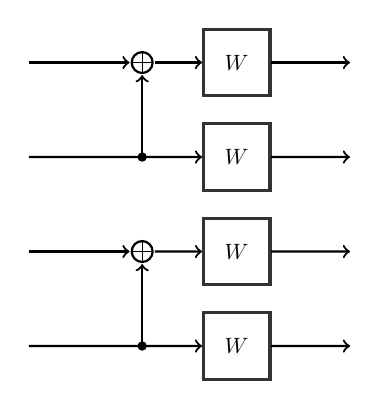
\begin{tikzpicture}[channel/.style={rectangle, draw=black!80, fill=white!5, very thick, minimum size=30}, scale=0.8, every node/.style={scale=0.8}]
                    \node[channel](channel1){$W$};
                    \node[channel](channel2) at (0, -1.5) {$W$};
                    \node[XOR, thick] at (-1.5, 0) {};
                    \node[circle, fill, inner sep = 1.5pt] at (-1.5, -1.5) {};
                    \draw[->, thick] (-3.3,0) to (-1.7, 0); 
                    \draw[->, thick] (-1.3,0) to (channel1.west); 
                    \draw[->, thick] (channel1.east) to (1.8, 0);
                    \draw[->, thick] (-3.3,-1.5) to (channel2.west); 
                    \draw[->, thick] (channel2.east) to (1.8, -1.5);
                    \draw[->, thick] (-1.5,-1.5) to (-1.5, -0.2); 
                    
                    \onslide<2>{
                    \node[channel](channel3) at (0, -3){$W$};
                    \node[channel](channel4) at (0, -4.5) {$W$};
                    \node[XOR, thick] at (-1.5, -3) {};
                    \node[circle, fill, inner sep = 1.5pt] at (-1.5, -4.5) {};
                    \draw[->, thick] (-3.3,-3) to (-1.7, -3); 
                    \draw[->, thick] (-1.3,-3) to (channel3.west); 
                    \draw[->, thick] (channel3.east) to (1.8, -3);
                    \draw[->, thick] (-3.3,-4.5) to (channel4.west); 
                    \draw[->, thick] (channel4.east) to (1.8, -4.5);
                    \draw[->, thick] (-1.5,-4.5) to (-1.5, -3.2); 
                    }
                \end{tikzpicture}
            }
            \only<3-9>{
            \begin{tikzpicture}[channel/.style={rectangle, draw=black!80, fill=white!5, very thick, minimum size=30}, scale=0.8, every node/.style={scale=0.8}]
                    \only<3-4>{
                    \node[channel](channel1){$W^-$};
                    \node[channel](channel2) at (0, -1.5) {$W^+$};
                    \node[channel](channel3) at (0, -3){$W^-$};
                    \node[channel](channel4) at (0, -4.5) {$W^+$};
                    }
                    \only<3,5->{
                    \draw[->, thick] (-3.3,0) to (channel1.west); 
                    \draw[->, thick] (-3.3,-1.5) to (channel2.west); 
                    }
                    \draw[->, thick] (-3.3,-3) to (channel3.west); 
                    \draw[->, thick] (channel3.east) to (1.8, -3);
                    \draw[->, thick] (-3.3,-4.5) to (channel4.west); 
                    \draw[->, thick] (channel4.east) to (1.8, -4.5);
                    \draw[->, thick] (channel1.east) to (1.8, 0);
                    \draw[->, thick] (channel2.east) to (1.8, -1.5);
                    
                    \onslide<4>{
                    \node[XOR, thick] at (-1.5, 0) {};
                    \draw[->, thick] (-3.3,0) to (-1.7, 0);
                    \draw[->, thick] (-1.3,0) to (channel1.west);
                    \node[XOR, thick] at (-2.5, -1.5) {};
                    \draw[->, thick] (-3.3,-1.5) to (-2.7, -1.5);
                    \draw[->, thick] (-2.3,-1.5) to (channel2.west);
                    \node[circle, fill, inner sep = 1.5pt] at (-1.5, -3) {};
                    \node[circle, fill, inner sep = 1.5pt] at (-2.5, -4.5) {};
                    \draw[->, thick] (-1.5,-3) to (-1.5, -0.2);
                    \draw[->, thick] (-2.5,-4.5) to (-2.5, -1.7);
                    }
                    \only<5->{
                    \node[channel](channel1){$W^{--}$};
                    \node[channel](channel2) at (0, -1.5) {$W^{+-}$};
                    \node[channel](channel3) at (0, -3){$W^{-+}$};
                    \node[channel](channel4) at (0, -4.5) {$W^{++}$};
                    }
                    
            \end{tikzpicture}
            }
            \only<10->{\includegraphics[width = 0.7\linewidth]{Figures/2stage-removebg-preview.jpg}
            \caption{Polarized Capacities for BEC(0.5) channel \cite{6852102}}}
        \end{figure}
    \end{column}
    
\end{columns}

\onslide<10-> Note that for $N = 2^t$ channels, we require $t$ stages of repeated polar transforms. We can see that the capacity of $W^{++}$ has improved significantly, while that of $W^{--}$ has deteriorated vastly \footnote<10->{Termed the \textbf{Matthew Effect:} The good become better and the bad get worse.}. \onslide<11->{\textcolor{red}{Are we approaching extremal polarization?}}
\end{frame}

\begin{frame}{Visualizing Polarization}
    \begin{figure}
        \centering
        \only<1>{\includegraphics[width = 0.6\linewidth]{Figures/N64.png}}
        \only<2>{\includegraphics[width = 0.6\linewidth]{Figures/N256.png}}
        \only<3>{\includegraphics[width = 0.6\linewidth]{Figures/N512.png}}
        \only<4>{\includegraphics[width = 0.6\linewidth]{Figures/N1024.png}}
        \only<1-4>{\caption{Distribution of capacities as polarization increases for BEC(0.4)}}
        \only<5>{\includegraphics[width = 0.8\linewidth]{Figures/PolarizationMartingale.jpg}\caption{Evolution of Polarization Martingale \cite{6852102}}        }
    \end{figure}
\end{frame}

\begin{frame}{Polarization Theorem}

\begin{theorem}
    As the number of channels $N = 2^t$ increases, the channel capacities $\left\{C(W_i)\right\}$ polarize. For any $\delta \in (0,1)$, 
    $$
    \frac{1}{N}\sum_{i=1}^{N} \mathbbm{1}\{C(W_i) > 1 - \delta\} \longrightarrow C(W)
    $$
    and
    $$
    \frac{1}{N}\sum_{i=1}^{N} \mathbbm{1}\{C(W_i) <  \delta\} \longrightarrow 1 - C(W)
    $$
\end{theorem}

\begin{itemize}
    \item<2-> The theorem tells us that, upon repeatedly applying polarization, the fraction of $\delta$-good channels converges to $C(W)$, and the fraction of $\delta$-bad channels converges to $1-C(W)$.
    \item<3-> As a corollary, we can see that the fraction of $\delta$-``mediocre'' channels, i.e. those with $C(W_i) \in (\delta, 1-\delta)$, converges to 0.
    \item<4-> This can be proven in a more general case by applying Doob's Martingale Convergence Theorem, and taking into account the fact that $\{ C(W_i) \}$ is a martingale bounded in $(0,1)$.
\end{itemize}
    
\end{frame}

\begin{frame}{Proof of Theorem (for BEC) - I}
    \begin{itemize}
        \item<1-> Let us quantify a particular behavior of a channel. For a BEC($p$) channel $W$, define $U(W) = \sqrt{p(1-p)}$.
        \item<2-> Observe that $U(W^+) = U(W)\sqrt{p(1+p)}$ and $U(W^-) = U(W)\sqrt{(1-p)(2-p)}$.
        \item<3-> Therefore $$\frac{1}{2}(U(W^+) + U(W^-)) = \frac{1}{2}U(W)(\sqrt{p(1+p)} + \sqrt{(1-p)(2-p)}) \leq \frac{\sqrt{3}}{2}U(W)$$.
        \item<4-> Expanding the sum
        $$
        \frac{1}{2^t}\sum_{i = 1}^{2^t}{U(W_i)} \leq \left(\frac{\sqrt{3}}{2}\right)^{t} U(W)
        $$
        \item<5-> We also have that 
        $$\mathbbm{1}\{C(W_i) \in (\delta, 1-\delta)\} \leq \frac{U(W_i)}{\sqrt{\delta(1-\delta)}}$$ 
    \end{itemize}
\end{frame}

\begin{frame}{Proof of Theorem (for BEC) - II}
    \begin{itemize}
        \item<1-> If we define the fraction of $\delta$-mediocre channels as $\mu_t (\delta)$, we have
        $$
        \mu_t (\delta) \coloneqq \frac{1}{2^t}\sum_{i = 1}^{2^t}{\mathbbm{1}\{C(W_i) \in (\delta, 1-\delta)\}}
        $$
        \item<2-> Therefore
        $$
        \mu_t (\delta) \leq \left(\frac{\sqrt{3}}{2}\right)^{t} \frac{U(W)}{\sqrt{\delta(1-\delta)}}
        $$
        \item<3-> So as the number of channels $N$ (and hence $t$) increases, this fraction goes to zero. 
        \item<4-> The fraction of perfect and useless channels follows trivially from the conservation of channel capacity.\\
        \hfill $\blacksquare$
    \end{itemize}
\end{frame}

\section{Encoding}

\begin{frame}{Encoding Scheme}
Suppose we wish to communicate at rate $R$:

\begin{itemize}
    \item<2-> Create $N = 2^t$ copies of the original channel $W$. We can apply the polarization transformation $t$ times to generate our $N$ synthetic channels.
    \item<3-> Select the $k = N\cdot R$ synthetic channels with the best polarized channel capacities, and set their inputs to be our information bits. Freeze the inputs of the remaining channels to some value (say 0). 
    \item<4-> Note that we can almost continuously adjust the rate of transmission by adding or deleting a polarized channel in use.
    \item<5-> Furthermore, the polarization theorem guarantees that, for large enough $N$, the fraction of perfect channels approaches $C(W)$. In such a scenario, we can reliably select these perfect channels to be our best ones to transmit information bits over. Therefore, we can achieve rates all the way up till the channel capacity.
\end{itemize}

\onslide<6->{
\begin{block}{Remark}
Unlike the goal of traditional code construction to maximize the minimum distance between codewords, polar coding aims to reduce the probability of error along information-bearing channels.
\end{block}
}
    
\end{frame}

\begin{frame}{Encoding Example}
\begin{columns}
    \begin{column}{0.3\linewidth}
    \onslide<4->{\begin{itemize}
        \item<4->Suppose we maintain a low tolerance of error, and we decide to use only the best three synthesized channels for transmitting data. Therefore, we have 
        $$
        \text{Rate} = \frac{3}{8} = 0.375
        $$
        \item<5->Our control over the rate can be seen more clearly if we decide to use the best 4 channels. In this case
        $$
        \text{Rate} = \frac{4}{8} = 0.5
        $$
    \end{itemize}}
    \end{column}
    \begin{column}{0.7\linewidth}
        \begin{figure}
        \centering
        
        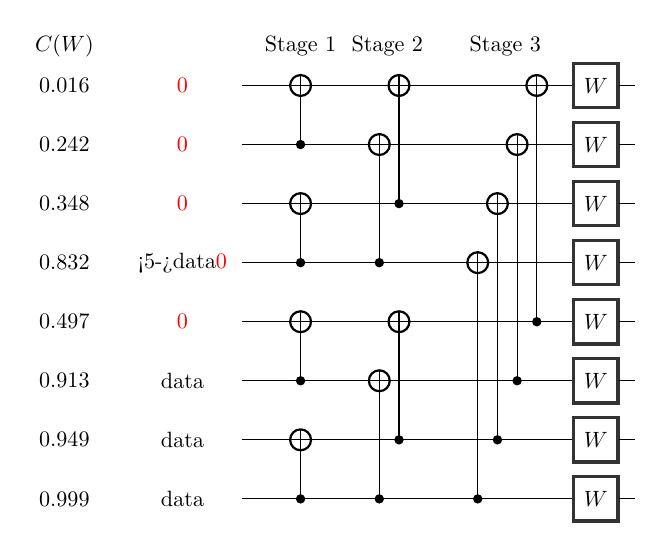
\begin{tikzpicture}[channel/.style={rectangle, draw=black!80, fill=white!5, very thick, minimum size=20}, scale=0.5, every node/.style={scale=0.8}]
            \node[channel](channel1) at (7.5, 0) {$W$};
            \node[channel](channel2) at (7.5, -1.5) {$W$};
            \node[channel](channel3) at (7.5, -3) {$W$};
            \node[channel](channel4) at (7.5, -4.5) {$W$};
            \node[channel](channel5) at (7.5, -6) {$W$};
            \node[channel](channel6) at (7.5, -7.5) {$W$};
            \node[channel](channel7) at (7.5, -9) {$W$};
            \node[channel](channel8) at (7.5, -10.5) {$W$};
            
            \node[] at (0, 1) {Stage 1};
            \node[] at (2.2, 1) {Stage 2};
            \node[] at (5.2, 1) {Stage 3};
            \onslide<2->{
            \node[] at (-6, 1) {$C(W)$};
            \node[] at (-6, 0) {0.016};
            \node[] at (-6, -1.5) {0.242};
            \node[] at (-6, -3) {0.348};
            \node[] at (-6, -4.5) {0.832};
            \node[] at (-6, -6) { 0.497};
            \node[] at (-6, -7.5) {0.913};
            \node[] at (-6, -9) {0.949};
            \node[] at (-6, -10.5) {0.999};
            }
            \onslide<3->{
            \node[] at (-3, 0) {\textcolor{red}{0}};
            \node[] at (-3, -1.5) {\textcolor{red}{0}};
            \node[] at (-3, -3) {\textcolor{red}{0}};
            \node[] at (-3, -4.5) {\alt<5->{data}{\textcolor{red}{0}}};
            \node[] at (-3, -6) {\textcolor{red}{0}};
            \node[] at (-3, -7.5) {data};
            \node[] at (-3, -9) {data};
            \node[] at (-3, -10.5) {data};
            }
        
            \node[XOR, thick] at (0, 0) {};
            \node[XOR, thick] at (0, -3) {};
            \node[XOR, thick] at (0, -6) {};
            \node[XOR, thick] at (0, -9) {};
            \node[circle, fill, inner sep = 1.5pt] at (0, -1.5) {};
            \node[circle, fill, inner sep = 1.5pt] at (0, -4.5) {};
            \node[circle, fill, inner sep = 1.5pt] at (0, -7.5) {};
            \node[circle, fill, inner sep = 1.5pt] at (0, -10.5) {};
            \draw[-] (0,-0.2) to (0, -1.5);
            \draw[-] (0,-3.2) to (0, -4.5);
            \draw[-] (0,-6.2) to (0, -7.5);
            \draw[-] (0,-9.2) to (0, -10.5);
            
            \node[XOR, thick] at (2.5, 0) {};
            \node[XOR, thick] at (2, -1.5) {};
            \node[XOR, thick] at (2.5, -6) {};
            \node[XOR, thick] at (2, -7.5) {};
            \node[circle, fill, inner sep = 1.5pt] at (2.5, -3) {};
            \node[circle, fill, inner sep = 1.5pt] at (2, -4.5) {};
            \node[circle, fill, inner sep = 1.5pt] at (2.5, -9) {};
            \node[circle, fill, inner sep = 1.5pt] at (2, -10.5) {};
            \draw[-] (2.5,-0.2) to (2.5, -3);
            \draw[-] (2, -1.7) to (2, -4.5);
            \draw[-] (2.5, -6.2) to (2.5, -9);
            \draw[-] (2, -7.7) to (2, -10.5);
            
            \node[XOR, thick] at (4.5, -4.5) {};
            \node[XOR, thick] at (5, -3) {};
            \node[XOR, thick] at (5.5, -1.5) {};
            \node[XOR, thick] at (6, 0) {};
            \node[circle, fill, inner sep = 1.5pt] at (4.5, -10.5) {};
            \node[circle, fill, inner sep = 1.5pt] at (5, -9) {};
            \node[circle, fill, inner sep = 1.5pt] at (5.5, -7.5) {};
            \node[circle, fill, inner sep = 1.5pt] at (6, -6) {};
            \draw[-] (4.5, -4.7) to (4.5, -10.5);
            \draw[-] (5, -3.2) to (5, -9);
            \draw[-] (5.5, -1.7) to (5.5, -7.5);
            \draw[-] (6, -0.2) to (6, -6);
            
            \draw[-] (-1.5, 0) to (channel1.west);
            \draw[-] (-1.5, -1.5) to (channel2.west);
            \draw[-] (-1.5, -3) to (channel3.west);
            \draw[-] (-1.5, -4.5) to (channel4.west);
            \draw[-] (-1.5, -6) to (channel5.west);
            \draw[-] (-1.5, -7.5) to (channel6.west);
            \draw[-] (-1.5, -9) to (channel7.west);
            \draw[-] (-1.5, -10.5) to (channel8.west);
            
            \draw[-] (channel1.east) to (8.5, 0);
            \draw[-] (channel2.east) to (8.5, -1.5);
            \draw[-] (channel3.east) to (8.5, -3);
            \draw[-] (channel4.east) to (8.5, -4.5);
            \draw[-] (channel5.east) to (8.5, -6);
            \draw[-] (channel6.east) to (8.5, -7.5);
            \draw[-] (channel7.east) to (8.5, -9);
            \draw[-] (channel8.east) to (8.5, -10.5);
            
        \end{tikzpicture}
        
        \caption{3-stage polar encoder for BEC(0.4)}
        
        \end{figure}
    \end{column}
\end{columns}    
\end{frame}




\begin{frame}{Encoding Complexity}
    \begin{columns}
    \begin{column}{0.6\linewidth}
    For a code of length $N = 2^t$,
    \begin{itemize}
        \item<1-> As noted, we will have $t$ polarization stages to synthesize our channels.
        \item<2-> Each polarization stage has $N/2$ \textbf{butterfly units} so as to cover all codeword indices. Each butterfly unit can carry out computation in $\mathcal{O}(1)$ time.
        \item<3-> Therefore, encoding complexity is $\mathcal{O}(t\cdot N)$, or $$\mathcal{O}(N \log N)$$
        
    \end{itemize}
    \end{column}
    \begin{column}{0.4\linewidth}
    \onslide<2->{
    \begin{figure}
        \centering
        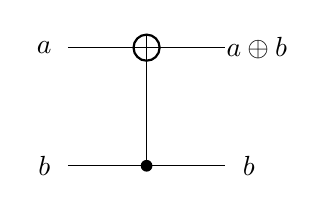
\begin{tikzpicture}
            \node[XOR, thick] at (0,0) {};
            \node[circle, fill, inner sep = 1.5pt] at (0, -1.5) {};
            \node[] at (-1.3, 0) {$a$};
            \node[] at (-1.3, -1.5) {$b$};
            \node[] at (1.4, 0) {$a \oplus b$};
            \node[] at (1.3, -1.5) {$b$};
            \draw[-] (0, -1.5) to (0, 0);
            \draw[-] (-1, 0) to (1, 0);
            \draw[-] (-1, -1.5) to (1, -1.5);
        \end{tikzpicture}
        \caption{Butterfly Unit}
    \end{figure}
    }
    
    \end{column}
    \end{columns}
    
\end{frame}

\section{Decoding}

\begin{frame}{Successive Cancellation Decoding}
    \begin{columns}
    \begin{column}{0.65\linewidth}
        \begin{columns}
        \begin{column}{0.5\linewidth}
        \onslide<1->{
        Looking at Stage 2
        \begin{itemize}
            \item $W^-: b_1 \to Y_1 Y_3$
            \item $W^-: b_2 \to Y_2 Y_4$
            \item $W^+: b_3 \to Y_1 Y_3 \hat{b_1}$
            \item $W^+: b_4 \to Y_1 Y_3 \hat{b_2}$\\
        \end{itemize}
        }
        \end{column}
        \begin{column}{0.5\linewidth}
        \onslide<2->{
        Looking at Stage 1
        \begin{itemize}
            \item $W^{--}: U_1 \to b_1 b_2$
            \item $W^{-+}: U_2 \to b_1 b_2 \hat{U_1}$
            \item $W^{+-}: U_3 \to b_3 b_4$
            \item $W^{++}: U_4 \to b_3 b_4 \hat{U_3}$\\
        \end{itemize}
        }
        \end{column}
        \end{columns}
    \vspace{10pt}
    \onslide<3->{
    Therefore, our channels can be represented as
    \begin{itemize}
        \item $W^{--}: U_1 \to Y_1 Y_2 Y_3 Y_4$
        \item $W^{-+}: U_2 \to Y_1 Y_2 Y_3 Y_4 \hat{U_1}$
        \item $W^{+-}: U_3 \to Y_1 Y_2 Y_3 Y_4 \alt<4->{\hat{U_1}\hat{U_2}}{\textcolor{red}{\hat{b_1}\hat{b_2}}}$
        \item $W^{++}: U_4 \to Y_1 Y_2 Y_3 Y_4 \alt<4->{\hat{U_1}\hat{U_2}}{\textcolor{red}{\hat{b_1}\hat{b_2}}} \hat{U_3}$
    \end{itemize}
    }
    \end{column}
    \begin{column}{0.35\linewidth}
        
    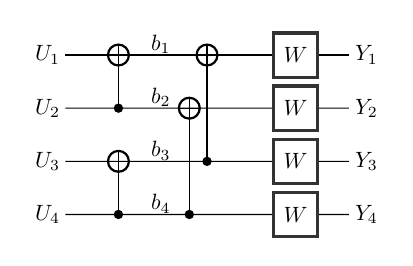
\begin{tikzpicture}[channel/.style={rectangle, draw=black!80, fill=white!5, very thick, minimum size=20}, scale=0.45, every node/.style={scale=0.8}]
            \node[channel](channel1) at (5, 0) {$W$};
            \node[channel](channel2) at (5, -1.5) {$W$};
            \node[channel](channel3) at (5, -3) {$W$};
            \node[channel](channel4) at (5, -4.5) {$W$};
            
            \node[] at (7, 0) {$Y_1$};
            \node[] at (7, -1.5) {$Y_2$};
            \node[] at (7, -3) {$Y_3$};
            \node[] at (7, -4.5) {$Y_4$};
            \node[] at (-2, 0) {$U_1$};
            \node[] at (-2, -1.5) {$U_2$};
            \node[] at (-2, -3) {$U_3$};
            \node[] at (-2, -4.5) {$U_4$};
            \node[] at (1.2, 0.3) {$b_1$};
            \node[] at (1.2, -1.2) {$b_2$};
            \node[] at (1.2, -2.7) {$b_3$};
            \node[] at (1.2, -4.2) {$b_4$};
        
            \node[XOR, thick] at (0, 0) {};
            \node[XOR, thick] at (0, -3) {};
            \node[circle, fill, inner sep = 1.5pt] at (0, -1.5) {};
            \node[circle, fill, inner sep = 1.5pt] at (0, -4.5) {};
            \draw[-] (0,-0.2) to (0, -1.5);
            \draw[-] (0,-3.2) to (0, -4.5);
            
            \node[XOR, thick] at (2.5, 0) {};
            \node[XOR, thick] at (2, -1.5) {};
            \node[circle, fill, inner sep = 1.5pt] at (2.5, -3) {};
            \node[circle, fill, inner sep = 1.5pt] at (2, -4.5) {};
            \draw[-] (2.5,-0.2) to (2.5, -3);
            \draw[-] (2, -1.7) to (2, -4.5);
            
            
            \draw[-] (-1.5, 0) to (channel1.west);
            \draw[-] (-1.5, -1.5) to (channel2.west);
            \draw[-] (-1.5, -3) to (channel3.west);
            \draw[-] (-1.5, -4.5) to (channel4.west);
            
            \draw[-] (channel1.east) to (6.5, 0);
            \draw[-] (channel2.east) to (6.5, -1.5);
            \draw[-] (channel3.east) to (6.5, -3);
            \draw[-] (channel4.east) to (6.5, -4.5);
            
        \end{tikzpicture}
        
    \end{column}
    \end{columns}
\end{frame}

\begin{frame}{Algorithm and Complexity}
    \begin{itemize}
        \item<1-> Decoding can be done using maximum likelihood decision making. \\
        \begin{columns}
            \begin{column}{0.5\linewidth}
            $$
            L^{--} = \frac{\mathbb{P}\{Y_1 Y_2 Y_3 Y_4 | U_1 = 0\}}{\mathbb{P}\{Y_1 Y_2 Y_3 Y_4 | U_1 = 1\}}
            $$
            $$
            \hat{U_1} = \begin{cases}
            0& \text{if } U_1 \text{ is frozen}\\
            0& \text{if } L^{--} > 1\\
            1& \text{otherwise}
            \end{cases}
            $$
            \end{column}
            \begin{column}{0.5\linewidth}
             $$
            L^{-+} = \frac{\mathbb{P}\{Y_1 Y_2 Y_3 Y_4 \hat{U_1}| U_2 = 0\}}{\mathbb{P}\{Y_1 Y_2 Y_3 Y_4 \hat{U_1}| U_2 = 1\}}
            $$
            $$
            \hat{U_2} = \begin{cases}
            0& \text{if } U_2 \text{ is frozen}\\
            0& \text{if } L^{-+} > 1\\
            1& \text{otherwise}
            \end{cases}
            $$
            \end{column}
        \end{columns}
        Decisions for $\hat{U_3}$ and $\hat{U_4}$ follow similarly.
        \item<2-> We have $t = \log N$ stages, and at each stage we make $N$ estimations. Therefore, our decoding complexity is 
        $$
        \mathcal{O}(N \log N)
        $$
    \end{itemize}
\end{frame}

\appendix
\section*{References}
\begin{frame}{References}
\bibliographystyle{ieeetr}
  \bibliography{references}
\vspace{10pt}
\textbf{Relevant Resources:}
\begin{itemize}
    \item \href{https://www.youtube.com/watch?v=VhyoZSB9g0w}{\textcolor{blue}{The Flesh of Polar Codes, ISIT 2017}} 
    \item \href{https://www.youtube.com/watch?v=PNBFUV-ZetY}{\textcolor{blue}{Polar Coding Tutorial, Arıkan}}
\end{itemize}

\end{frame}

\section*{Algebra}

\begin{frame}{Algebraic Formulation}
    \begin{columns}
        \begin{column}{0.4\linewidth}
        \begin{itemize}
            \item<4-> Define
            $$
            F_2 = \begin{bmatrix} 1 & 0\\ 1 & 1 \end{bmatrix}
            $$
            \item<5-> Then, for $N = 2^t$,
            $$
            F_{2N} = \begin{bmatrix} F_N & 0\\ F_N & F_N \end{bmatrix}
            $$
            \item<6-> Therefore, the generator matrix for a $N = 2^t$ length polar code is
            $$
            G_N = B_N F_N
            $$
            where $B_N$ is a bit-reversal permutation matrix.
        \end{itemize}
        \end{column}
        \begin{column}{0.6\linewidth}
        \only<1>{
        \begin{figure}
            \centering
            \includegraphics[width = 0.6\linewidth]{Figures/W4.jpg}
            \caption{Symmetric block diagram for 2-stage polarizer \cite{5075875}}
        \end{figure}
        }
        \only<2>{
        \begin{figure}
            \centering
            \includegraphics[width = 0.6\linewidth]{Figures/WN.jpg}
            \caption{Symmetric block diagram for general polarizer \cite{5075875}}
        \end{figure}
        }
        \onslide<3->{
        \begin{figure}
            \centering
            \includegraphics[width = 0.6\linewidth]{Figures/WN_alt.jpg}
            \caption{Alternate block diagram for general polarizer \cite{5075875}}
        \end{figure}
        }
        \end{column}
    \end{columns}
\end{frame}

\end{document}



